
\section{Các máy Turing}
\label{sec:112}
Trong nỗ lực để hiểu khả năng và giới hạn của máy tính, nhiều nhà nghiên cứu đã đề xuất và
nghiên cứu nhiều thiết bị tính toán khác nhau. Một trong số đó là máy Turing, được đề xuất
bởi Alan~M.~Turing từ năm $1936$ và ngày nay nó vẫn được dùng như một công cụ để nghiên
cứu khả năng của quá trình thuật toán.

\subsection*{Cơ bản về máy Turing}
Một \textbf{máy Turing} bao gồm một đơn vị điều khiển có thể đọc và ghi các ký hiệu trên
một băng dùng một đầu đọc/ghi (Hình~\ref{fig:fig112}). Băng này có thể mở rộng vô hạn về
cả hai phía và nó được chia thành các ô, mỗi ô có thể chứa một phần tử thuộc một tập hữu
hạn các ký hiệu. Tập này được gọi là bộ chữ của máy.

\begin{figure}[bht]
  \centering 
  \scalebox{0.4}{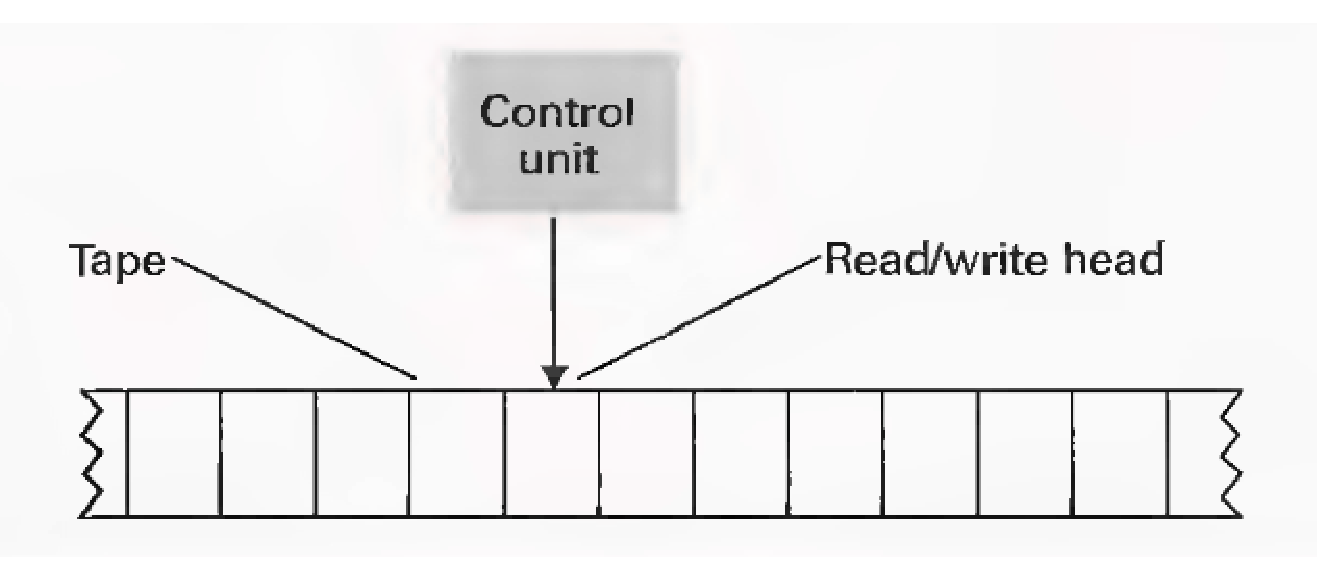
\includegraphics{ch7/fig112.pdf}}
  \caption{Các thành phần của một máy Turing}
\label{fig:fig112}
\end{figure}

Tại mỗi thời điểm tính toán, máy Turing ở một trạng thái nào đó và số trạng thái của máy
là hữu hạn. Một tính toán của máy Turing bắt đầu ở một trạng thái đặc biệt được gọi là
trạng thái bắt đầu và máy dừng khi đạt đến một trạng thái đặc biệt, gọi là trạng thái
dừng.


Một tính toán của máy Turing bao gồm một dãy các bước được thực hiện bởi đơn vị điều
khiển. Mỗi bước bao gồm việc quan sát ký hiệu ở ô hiện hành (ô này được nhìn bởi đầu
đọc/ghi) trên băng, viết một ký hiệu lên ô, có khả năng chuyển đầu đọc sang ô bên trái
hoặc bên phải, và sau đó thay đổi trạng thái. Hoạt động máy phải thực hiện được xác định
bởi một chương trình, nó dựa vào trạng thái của máy và nội dung của ô nhớ hiện thời trên
băng để chỉ ra đơn vị điều khiển phải làm gì .

Ta cùng xem xét một ví dụ về một máy Turing. Để tiện lợi, ta biểu diễn băng của máy như
một đường thẳng nằm ngang chia thành các ô. Trên mỗi ô này ta có thể ghi một ký hiệu thuộc
bảng chữ của máy. Ta chỉ ra vị trí hiện thời của đầu đọc/ghi bằng cách đặt một nhãn dưới ô
nhớ hiện thời. Bộ chữ máy trong ví dụ của ta bao gồm các ký hiệu $0,1$ và $*$. Băng của
máy có thể xuất hiện như sau:
\begin{center}
   \scalebox{0.45}{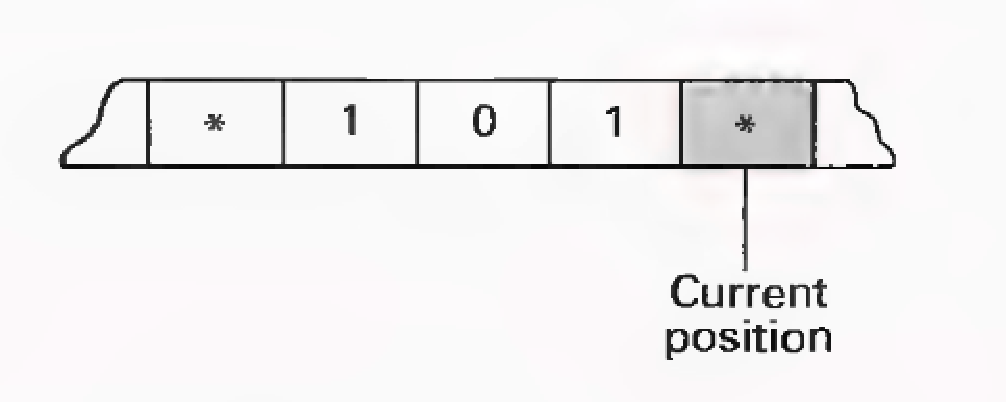
\includegraphics{ch7/turing1.pdf}}
\end{center}
%\end{wrapfigure}

Bằng cách diễn giải xâu ký hiệu trên băng như các biểu diễn nhị phân của các số nguyên
được ngăn cách bởi các dấu sao, ta thấy băng ở trên chứa giá trị $5$. Máy Turing của ta sẽ
được thiết kế để tăng giá trị trên băng lên $1$. Nói chính xác hơn, nó giả sử rằng vị trí
bắt đầu tại dấu sao bên phải của xâu gồm $0$ và $1$, và nó thực hiện biến đổi xâu thành
xâu biểu diễn số nguyên tiếp theo.

Các trạng thái của máy là \texttt{START}, \texttt{ADD}, \texttt{CARRY}, \texttt{OVERFLOW},
\texttt{RETURN}, và \texttt{HALT}. Các hoạt động tương ứng với mỗi trạng thái và nội dung
của ô hiện hành được mô tả theo bảng trong trong Hình~\ref{fig:fig113}.
 
Ta cùng chạy máy này trên băng biểu diễn giá trị $5$ trong hình trước. Máy bắt đầu ở trạng
thái \texttt{START} và ô nhớ hiện thời chứa $*$. Ta thực hiện theo chỉ dẫn ở bảng trên:
ghi lại giá trị $*$, chuyển đầu đọc/ghi sang trái một ô, và máy chuyển sang trạng thái
\texttt{ADD}. Máy bây giờ được mô tả như dưới đây:
\begin{center}
   \scalebox{0.45}{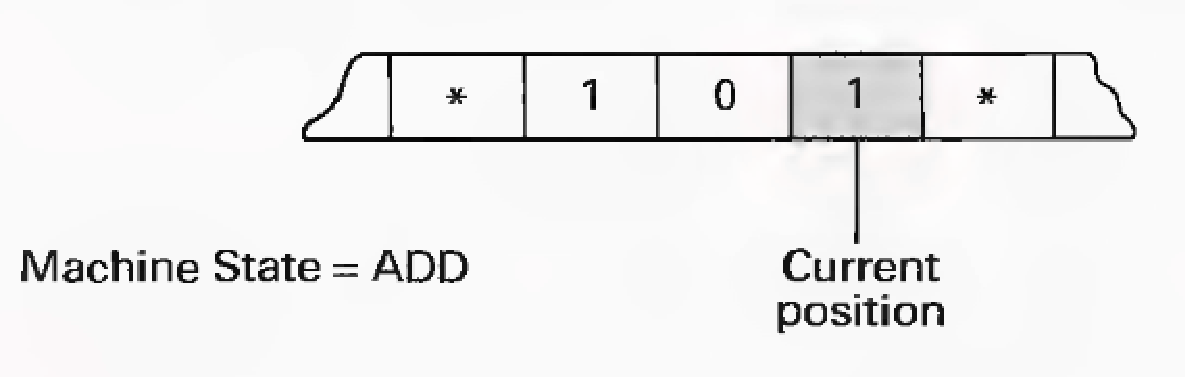
\includegraphics{ch7/turing2.pdf}}
\end{center}


Ta tiếp tục nhìn bảng trên để xem phải làm gì khi máy ở trạng thái \texttt{ADD} và ô hiện
tại chứa giá trị $0$. Bảng trên chỉ ra: thay thế $1$ ở ô nhớ hiện tại bởi $0$, chuyển đầu
đọc/ghi sang trái một ô, và máy chuyển sang trạng thái \texttt{CARRY}. Bây giờ hình trạng
của máy trở thành:
\begin{center}
   \scalebox{0.45}{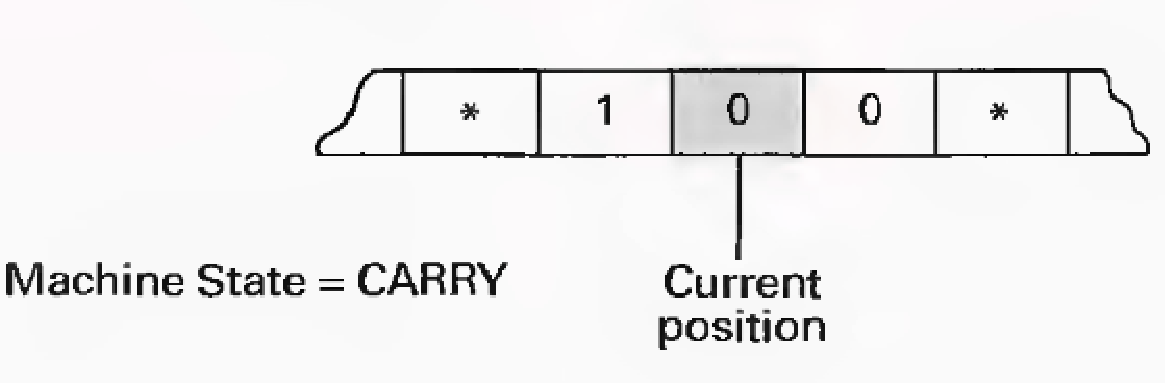
\includegraphics{ch7/turing3.pdf}}
\end{center}

Ta lại xem bảng trên để xem phải làm gì tiếp và thấy rằng khi máy ở trạng thái
\texttt{CARRY} với ô hiện hành chứa $0$, ta phải thay $0$ bằng $1$, chuyển đầu đọc/ghi
sang phải, và máy chuyển sang trạng thái \texttt{RETURN}. Bây giờ hình trạng của máy như
sau:
\begin{center}
   \scalebox{0.45}{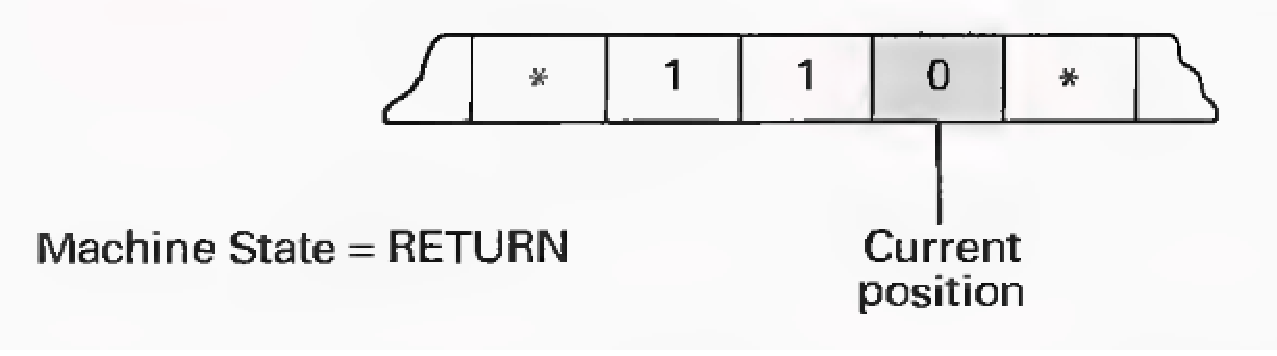
\includegraphics{ch7/turing4.pdf}}
\end{center}


Từ tình huống này, bảng trước chỉ ra ta phải thay $0$ ở ô hiện thời với giá trị $0$ khác,
chuyển đầu đọc/ghi sang phải, và máy vẫn ở trạng thái \texttt{RETURN}. Vậy máy ở trong
điều kiện sau đây:
\begin{center}
   \scalebox{0.45}{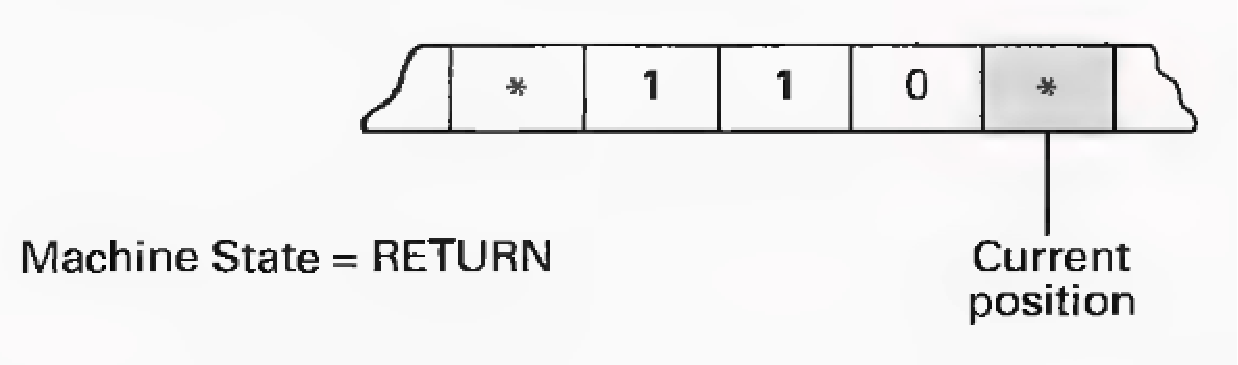
\includegraphics{ch7/turing5.pdf}}
\end{center}

Tại thời điểm này, ta thấy bảng trên chỉ ra rằng viết lại dấu sao trong ô hiện thời và máy
chuyển sang trạng thái \texttt{HALT}. Vậy máy dừng ở hình trạng sau đây (các ký hiệu trên
băng bây giờ biểu diễn giá trị $6$ đúng như ta mong đợi):
\begin{center}
   \scalebox{0.45}{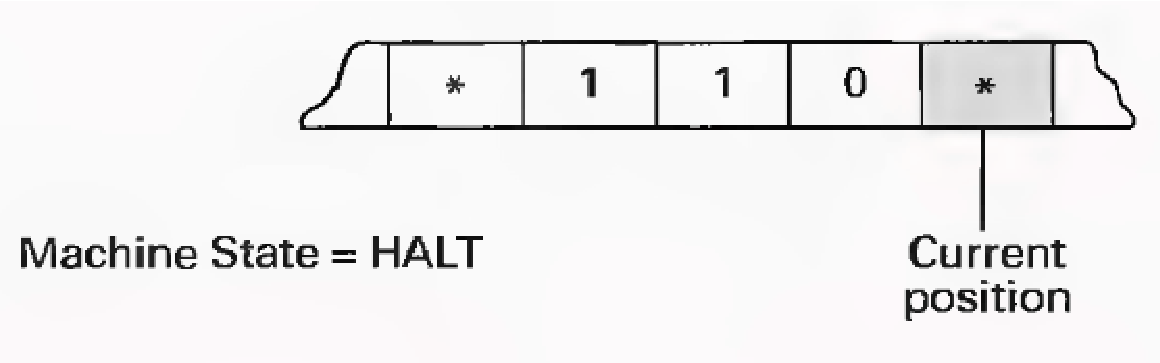
\includegraphics{ch7/turing6.pdf}}
\end{center}


\begin{figure}
  \label{fig:fig113}  
  \centering
  \begin{tabular}{ccccc} \hline
    \textbf{Trạng thái} & \textbf{Nội dung ô nhớ} & \textbf{Giá trị} & \textbf{Hướng di chuyển} & \textbf{Trạng thái} \\
    \textbf{hiện thời}  & \textbf{hiện thời}      & \textbf{cần ghi} &                          & \textbf{tiếp theo}  \\
    \hline
    \texttt{START}      & $*$                     & $*$              & sang Trái                & \texttt{ADD}        \\
    \texttt{ADD}        & $0$                     & $1$              & sang Phải                & \texttt{RETURN}     \\
    \texttt{ADD}        & $1$                     & $0$              & sang Trái                & \texttt{CARRY}      \\
    \texttt{ADD}        & $*$                     & $*$              & sang Phải                & \texttt{HALT}       \\
    \texttt{CARRY}      & $0$                     & $1$              & sang Phải                & \texttt{RETURN}     \\
    \texttt{CARRY}      & $1$                     & $0$              & sang Trái                & \texttt{CARRY}      \\
    \texttt{CARRY}      & $*$                     & $1$              & sang Trái                & \texttt{OVERFLOW}   \\
    \texttt{OVERFLOW}   & $*$                     & $*$              & sang Phải                & \texttt{RETURN}     \\
    \texttt{RETURN}     & $0$                     & $0$              & sang Phải                & \texttt{RETURN}     \\
    \texttt{RETURN}     & $1$                     & $1$              & sang Phải                & \texttt{RETURN}     \\
    \texttt{RETURN}     & $*$                     & $*$              & không chuyển             & \texttt{HALT}       \\
    \hline
  \end{tabular}
  \caption{Một máy Turing tăng giá trị}
\end{figure}

\subsection*{Luận đề Church-Turing}
Máy Turing trong phần trước được sử dụng để tính hàm tìm số liền sau, gắn mỗi giá trị đầu
vào là số nguyên không âm $n$ với giá trị đầu ra $n + 1$. Công việc của ta đơn thuần chỉ
là chuyển giá trị đầu vào thành dạng nhị phân và đặt lên băng của máy, để máy chạy cho tới
khi nó dừng, và sau đó đọc giá trị đầu ra trên băng. Một hàm có thể được tính bởi máy
Turing theo cách này được gọi là \textbf{tính được bằng máy Turing}.

Giả thiết của Turing là các hàm tính được bằng máy Turing cũng chính là các hàm tính
được. Nói cách khác, ông giả sử rằng khả năng tính toán của máy Turing chứa mọi hệ thống
thuật toán. Hay tương đương, mọi hàm tính được đều là hàm tính được bởi một máy Turing nào
đó. Giả thuyết này ngày nay được gọi là \textbf{luận đề Church-Turing}, để tưởng nhớ tới
các đóng góp của Alan~Turing và Alonzo~Church. Luận đề này không được chứng minh chặt chẽ
bằng toán học, tuy nhiên cho đến nay thực tiễn luôn chứng minh rằng luận đề đó là đúng đắn
và được chấp nhận rộng rãi. Có nghĩa rằng, hàm tính được và các hàm tính được bởi máy
Turing được xem xét là trùng nhau.

Điều đáng chú ý của giả thuyết này là nó cho ta nhận thức về khả năng và giới hạn của
máy. Chính xác hơn, nó thiết lập khả năng của các máy Turing như một chuẩn để các hệ thống
tính toán khác có thể so sánh. Nếu một hệ thống nào đó có khả năng tính toán mọi hàm có
thể tính bới máy Turing, thì nó được xem như có khả năng mạnh nhất mà mọi hệ thống tính
toán có thể.

\subsection*{Câu hỏi \& Bài tập}
\begin{enumerate}
\item Chạy máy Turing được mô tả trong mục này (Hình~\ref{fig:fig113}), nhưng với trạng
  thái khởi đầu sau đây:
\begin{center}
   \scalebox{0.45}{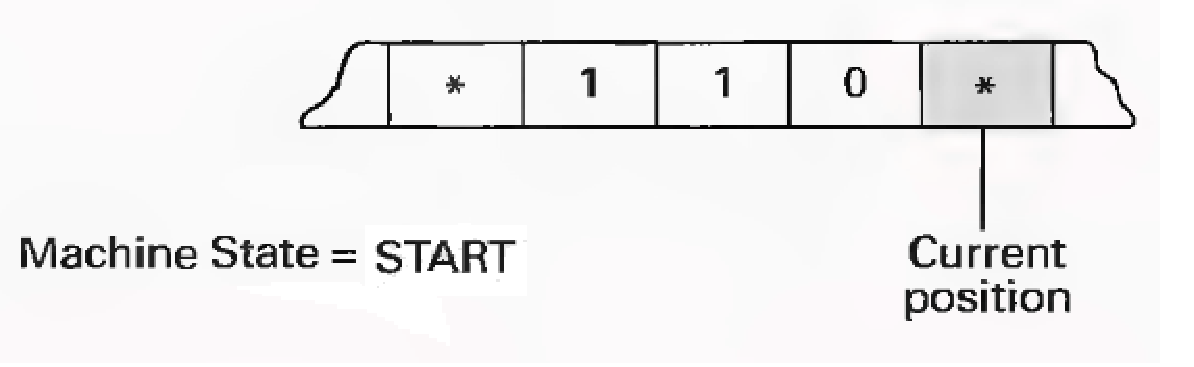
\includegraphics{ch7/turing7.pdf}}
\end{center}

\item Mô tả một máy Turing thay thế các xâu gồm các chữ $0$ và $1$ thành xâu chỉ gồm một
  chữ $0$.

\item Mô tả một máy Turing giảm giá trị trên băng đi một nếu giá trị đó lớn hơn không hoặc
  để nguyên nếu giá trị đó bằng không.

\item Chỉ ra một tình huống ngoài đời thường mà phải thực hiện tính toán. Tình huống này
  tương tự với một máy Turing như thế nào?

\item Mô tả một máy Turing dừng với một số đầu vào nhưng không bao giờ dừng với các đầu
  vào khác.
\end{enumerate}



%%% Local Variables: 
%%% mode: latex
%%% TeX-master: "../tindaicuong"
%%% End: 
